\documentclass{article} % For LaTeX2e
% We will use NIPS submission format
\usepackage{nips13submit_e,times}
% for hyperlinks
\usepackage{hyperref}
\usepackage{url}
% For figures
\usepackage{graphicx} 
\usepackage{subfigure} 
% math packages
\usepackage{amsmath}
\usepackage{amsfonts}
\usepackage{amsopn}
\usepackage{ifthen}
\usepackage{natbib}

\title{Project-I by Group OSLO}

\author{
Etienne Pot \and  Lucile Madoulaud\\
EPFL \\
\texttt{etienne.pot@epfl.ch  \and lucile.madoulaud@epfl.ch } \\
}

\date{
Nov 2015
}

\nipsfinalcopy

\begin{document}

\maketitle

This report present our method and prediction results of for the regression and classification tasks. For the regression task, we have decided to train three different models and a model selector, we obtain respectable performance except for some outliers which have too much impact on our RMSE. We discut about some improvement possible to solve this problem.
For the classification task, we have decided to train two different models this time.

\end{abstract}

\section{Data Description}
We have input test-data $\mathbf{X}$ which consists in$N=1200$ data of 65 variables for the regression. We also have train-data consists in an input and an output. These data are composed by $2800$ datas. The classification also contains 1500 test data  $\mathbf{X}$ and train data with output and output with only 29 variables.
In this project, we want to make some predictions for the test-data.

\section{Data visualization and cleaning}
First of all, we have done some exploration of our data before we start to apply a machine learning algorithm.
On the regression task, by plotting the histogram of the output (Figure \ref{fig:histY}), we can clearly see three distinct clusters, around 2000, 6000 and 12000.
We have also plotted each variable in function of the output to see if there was some variable directly correlated to our output. We have see for instance that the variables 16 and 38 could help us to discriminate between the three clusters (Figure \ref{fig:clusters}) and that for each cluster, there was a variable which was strongly linearly correlated with the output (12, 26 and 61), those could eventually be used to have a first really simple model with only one dimension.

\begin{figure}[!t]
\center
\subfigure[Histogram of $\mathbf{y}$. We clearly see three clusters.]{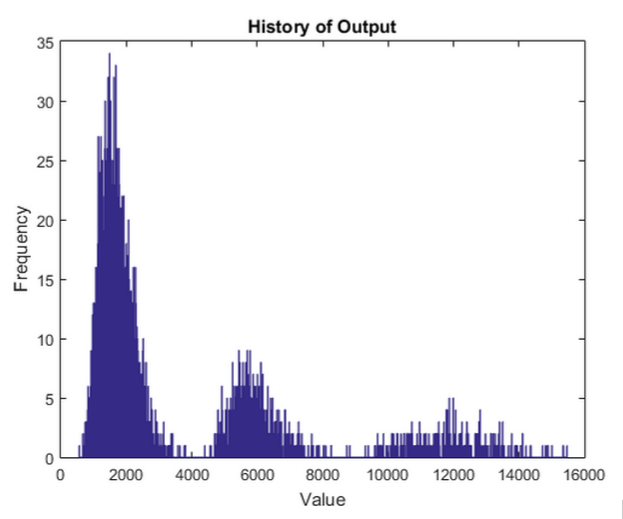
\includegraphics[width=2.5in]{figures/histY.jpg} \label{fig:histY}}
\hfill
\subfigure[Output in fonction of two interesting variables. The clusters are in evidence with their color]{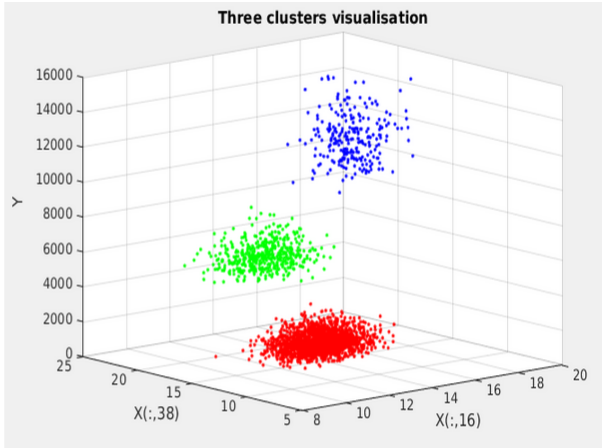
\includegraphics[width=2.5in]{figures/clusters.jpg} \label{fig:clusters}}
\caption{}
\end{figure}

Similarly, for the classification task, by plotting the histogram of the $\mathbf{X}$ (for instance column 10), we see that our input seems to be the sum of two gaussian distributions. We have also used those histogram to isolate and remove some outliers which were really far from the gaussian distributions.

\begin{figure}[!t]
\center
\subfigure[Histogram of variable 10 of $\mathbf{X}$. We see the two gaussian and some outliers. ]{\includegraphics{figures/hist.jpg} \label{fig:histY}}
\caption{}
\end{figure}

\subsubsection*{References}

\end{document}
